\documentclass[a4paper,12pt]{article}
\usepackage[utf8]{inputenc}
\usepackage{cmap}
\usepackage[T2A]{fontenc}
\usepackage[english,russian]{babel}
\usepackage{amsmath,amssymb,mathtools}
\usepackage{graphicx,float,caption,booktabs}
\usepackage{subcaption}
\usepackage{textcomp}
\setlength{\topmargin}{-0.5in}
\setlength{\textheight}{9.1in}
\setlength{\oddsidemargin}{-0.4in}
\setlength{\evensidemargin}{-0.4in}
\setlength{\textwidth}{7in}
\setlength{\parindent}{0ex}
\setlength{\parskip}{1ex}
\DeclareCaptionLabelSeparator{defffis}{ --- }
\captionsetup{justification=centering,labelsep=defffis}
\usepackage[unicode,hidelinks]{hyperref}
\title{Лабораторная работа № 1\\Итерационные методы решения\\разреженных СЛАУ и предобуславливание\\Вариант H1}
\author{Соложенкин Севастьян, Б01-411}
\date{}
\begin{document}
\maketitle
\newpage

\section{Физическая постановка задачи}
Рассматривается стационарное распределение температуры в квадратной пластине с неоднородной теплопроводностью. Вблизи центра действует локализованный источник тепла; температура на всех сторонах пластины поддерживается равной нулю. Требуется найти температурное поле и оценить его максимум.

\section{Математическая постановка}
Для области $\Omega=(0,1)^2$ решается краевая задача
\begin{equation}
    -\nabla\!\cdot\!\bigl(a(x,y)\nabla u\bigr)+c(x,y)u=f(x,y),
    \qquad u\big|_{\partial\Omega}=0,
    \label{eq:pde}
\end{equation}
где
\begin{align*}
    a(x,y) & =1+0.35\sin(2\pi x)\sin(2\pi y),                                 & c(x,y) & =0, \\
    f(x,y) & =30\exp\!\left(-\frac{(x-0.5)^2+(y-0.5)^2}{2\cdot0.12^2}\right).
\end{align*}
Так как $0.65\leq a\leq1.35$, коэффициент теплопроводности положителен. Задача стационарная, поэтому начальные условия не задаются.

Используется равномерная сетка $N\times N$ с шагом $h=1/(N-1)$. Потоки через грани ячеек аппроксимируются центральными разностями, а $a$ в середине ребра --- средним значением в соседних узлах. Получается симметричная пятидиагональная по шаблону система $Au=b$ с $n=(N-2)^2$ внутренними неизвестными; матрица хранится в формате CSR. На тестовой сетке $N=8$ симметричность и положительная определённость подтверждены проверками и разложением Холецкого.

\section{Методы численного решения}
Реализованы стационарные методы Якоби, Гаусса--Зейделя и последовательной верхней релаксации (ПВР), а также метод сопряжённых градиентов (CG) и предобусловленный CG (PCG) с диагональным и SSOR-предобуславливателями. Для ПВР использовано $\omega=1.9075$, найденное перебором на сетке $N=64$ (230 итераций). Для SSOR-PCG параметр подобран отдельно по минимальному числу итераций на сетке $N=64$: проверены 16 значений $\omega\in[0.5,1.95]$ и 21 значение при уточнении в окрестности лучшего. Получено $\omega=1.7067$ (30 итераций).

Начальное приближение $u^{(0)}=0$. Критерий остановки --- истинная относительная невязка
\begin{equation}
    \eta_s=\frac{\|b-Au^{(s)}\|_2}{\|b\|_2}\leq10^{-8}.
    \label{eq:residual}
\end{equation}
Корректность проверена на искусственной системе с известным решением $b^*=Au^*$; для основной системы использовано независимое сравнение с разреженным прямым решателем \texttt{spsolve} в относительных нормах $L_2$ и $L_\infty$. Времена --- медианы трёх запусков после прогрева, при одном потоке BLAS. Для CG/PCG время подготовки предобуславливателя измеряется отдельно от времени итераций.

\section{Результаты вычислений}
\begin{table}[H]
    \centering
    \caption{Размер и обусловленность дискретных систем}
    \begin{tabular}{rrrrr}
        \toprule
        $N$ & $n$     & $\mathrm{nnz}(A)$ & $\kappa_2(A)$ & CSR, MB \\
        \midrule
        32  & 900     & 4\,380            & 504.2         & 0.056   \\
        64  & 3\,844  & 18\,972           & 2\,137.4      & 0.243   \\
        128 & 15\,876 & 78\,876           & 8\,797.8      & 1.010   \\
        \bottomrule
    \end{tabular}
\end{table}
\begin{table}[H]
    \centering
    \caption{Число итераций до $\eta_s\leq10^{-8}$ и время на сетке $N=128$}
    \begin{tabular}{lrrrr}
        \toprule
        Метод                       & $N=32$      & $N=64$      & $N=128$     & Время $N=128$, мс \\
        \midrule
        Якоби                       & 3\,547      & 14\,667     & 59\,624     & 3\,317.8          \\
        Зейдель                     & 1\,775      & 7\,335      & 29\,813     & 6\,494.4          \\
        ПВР ($\omega=1.9075$)       & 205         & 230         & 1\,368      & 283.6             \\
        CG                          & 67          & 147         & 311         & 34.1              \\
        PCG, диагональный           & 62          & 130         & 266         & \textbf{31.5}     \\
        PCG, SSOR ($\omega=1.7067$) & \textbf{22} & \textbf{30} & \textbf{51} & 98.0              \\
        \bottomrule
    \end{tabular}
\end{table}

\noindent\textbf{Независимая проверка.} Относительная невязка контрольного решения \texttt{spsolve} на сетках $N=32,64,128$ составляет $2.15\cdot10^{-14}$, $9.84\cdot10^{-14}$ и $3.97\cdot10^{-13}$ соответственно. Для всех реализованных методов относительные различия с контрольным решением в нормах $L_2$ и $L_\infty$ не превышают $1.4\cdot10^{-8}$.

\begin{figure}[H]
    \centering
    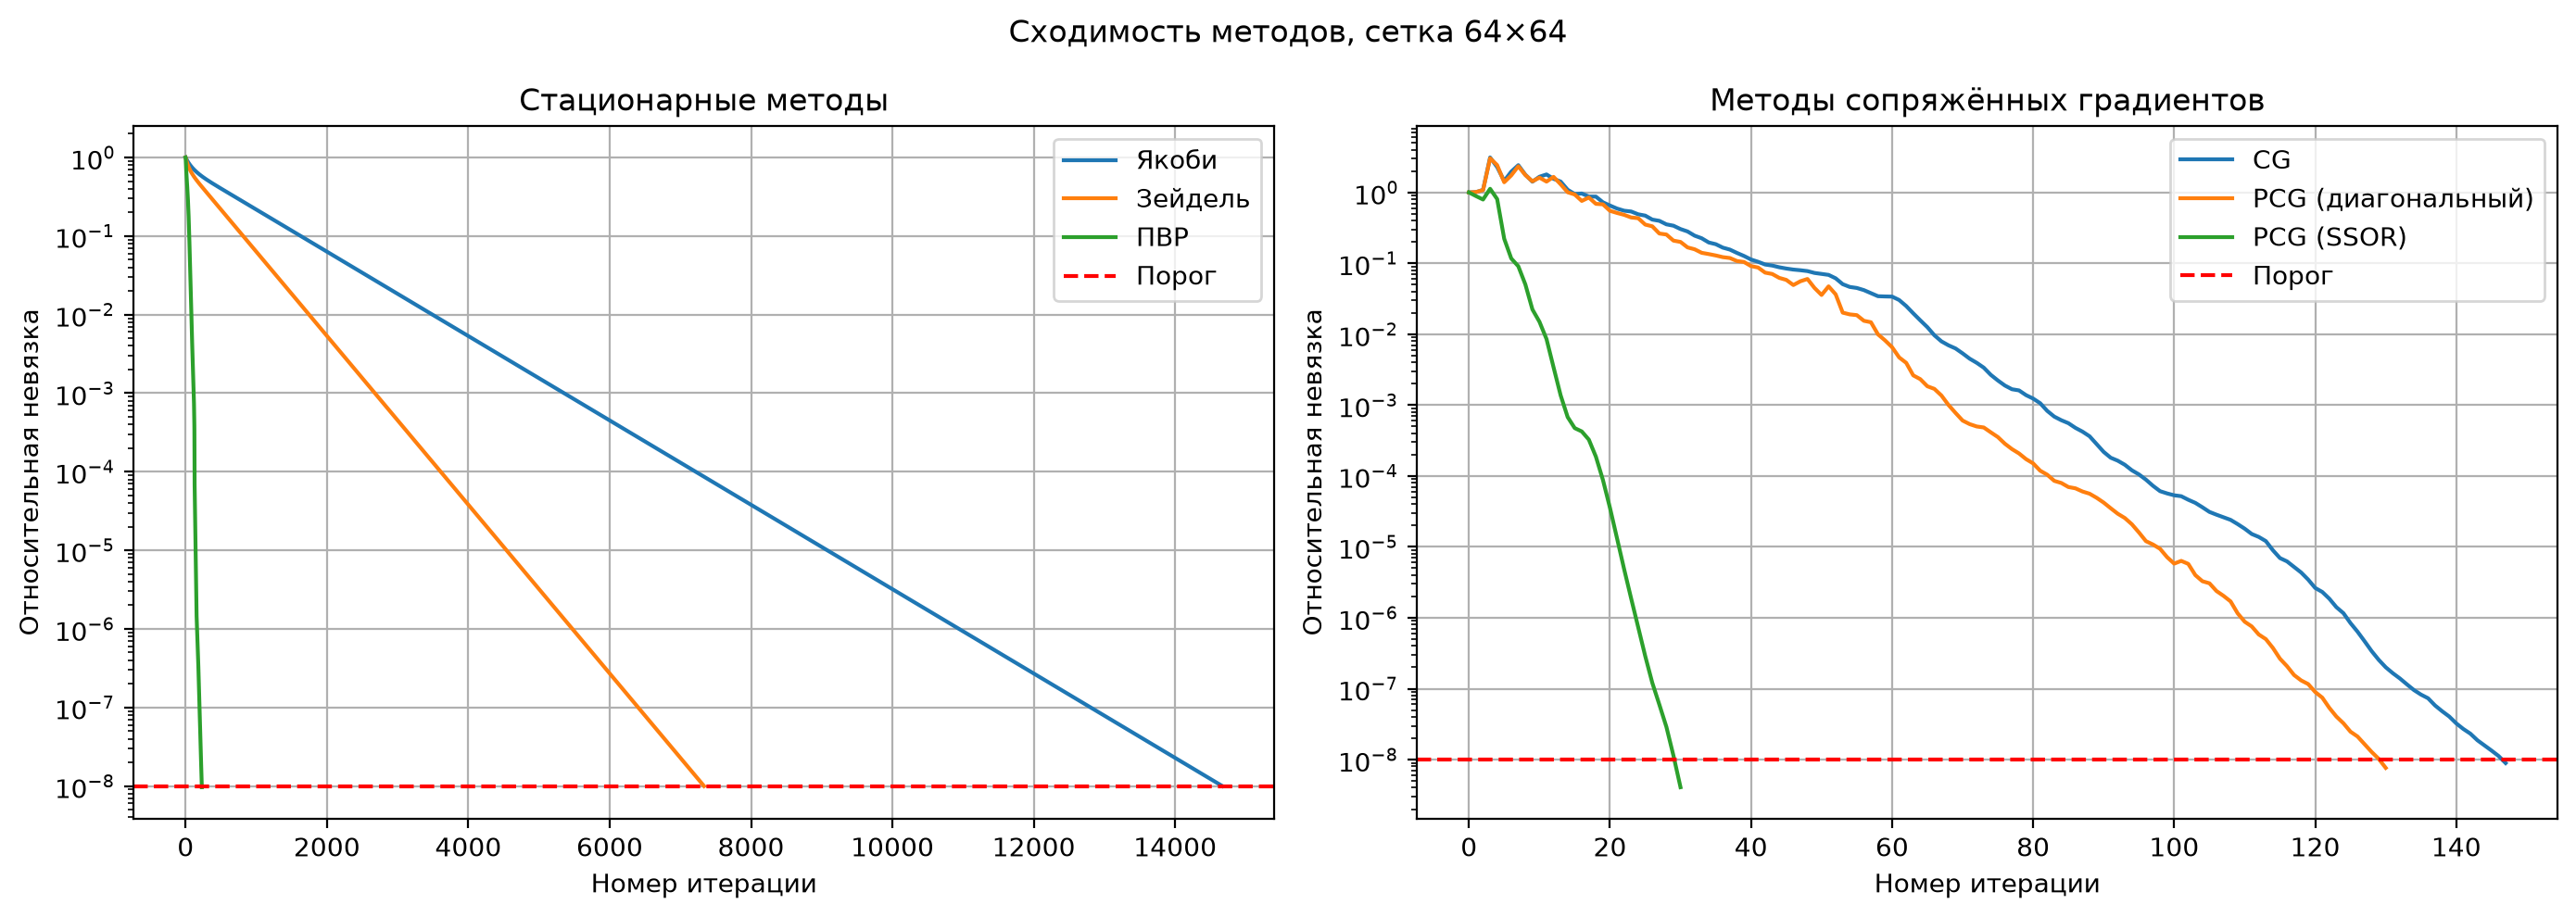
\includegraphics[width=0.96\linewidth]{figures/residual_histories.png}
    \caption{Истории истинной относительной невязки на сетке $N=64$ (логарифмическая шкала).}
\end{figure}

\begin{figure}[H]
    \centering
    \begin{subfigure}[t]{0.46\linewidth}
        \centering
        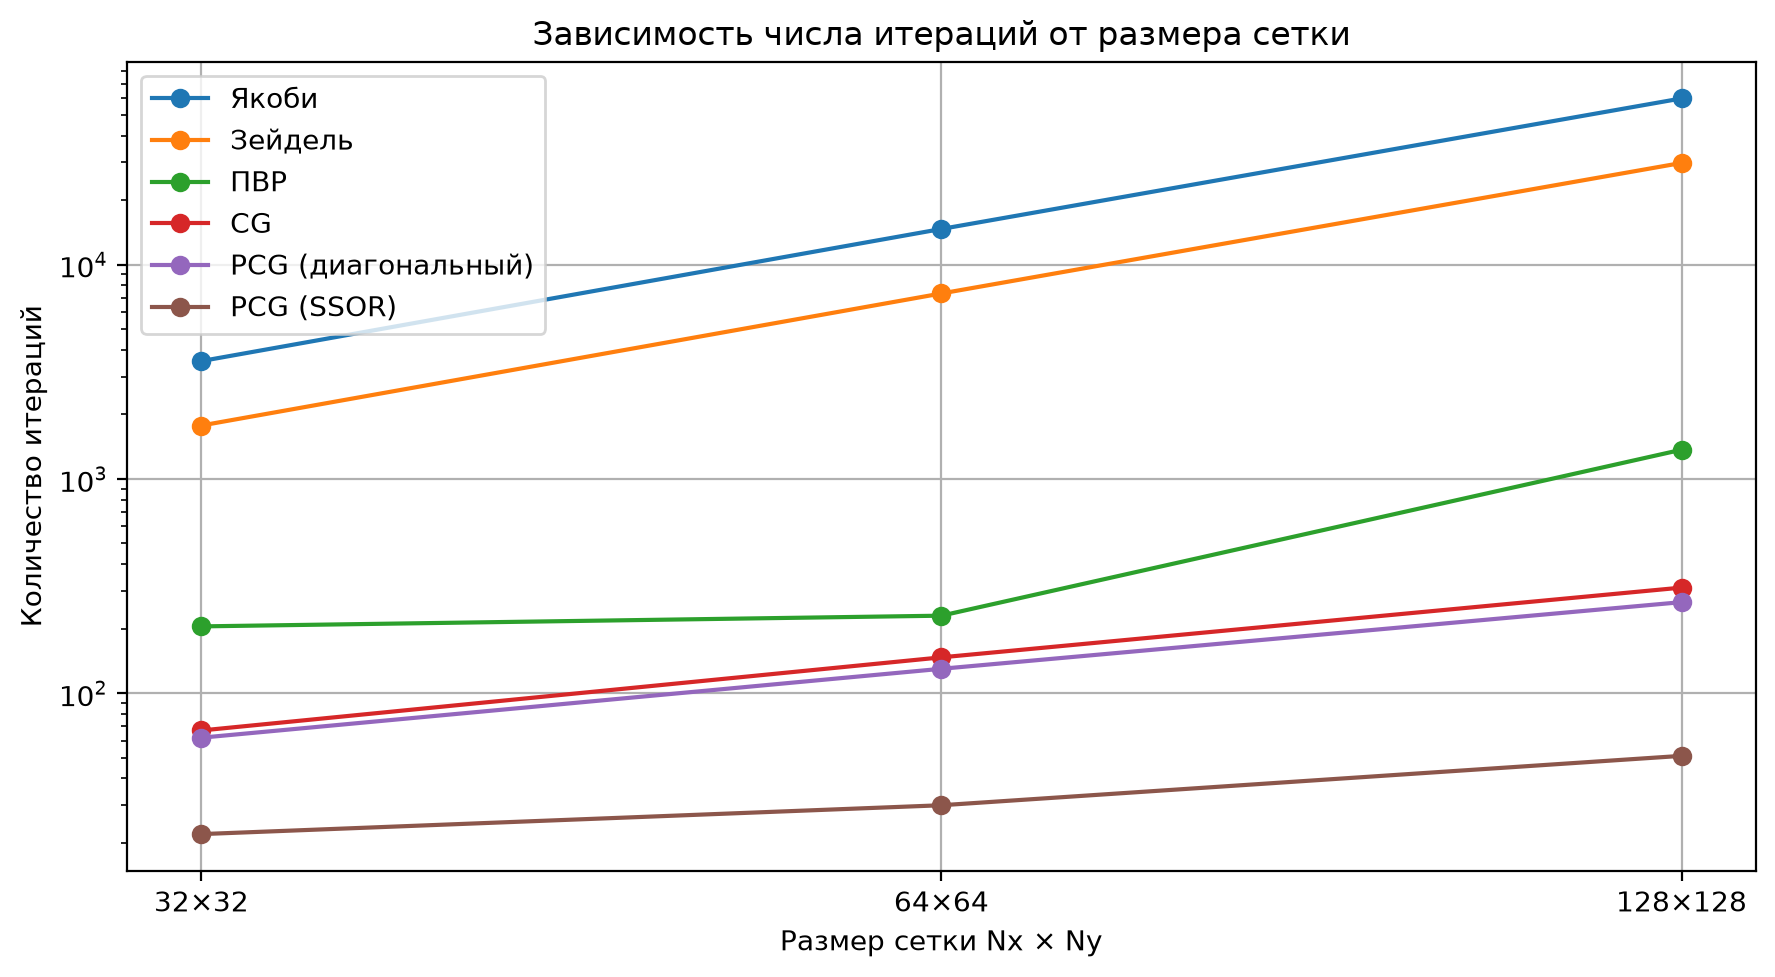
\includegraphics[width=\linewidth]{figures/iteration_counts.png}
        \caption{Число итераций в зависимости от $N$.}
    \end{subfigure}\hfill
    \begin{subfigure}[t]{0.46\linewidth}
        \centering
        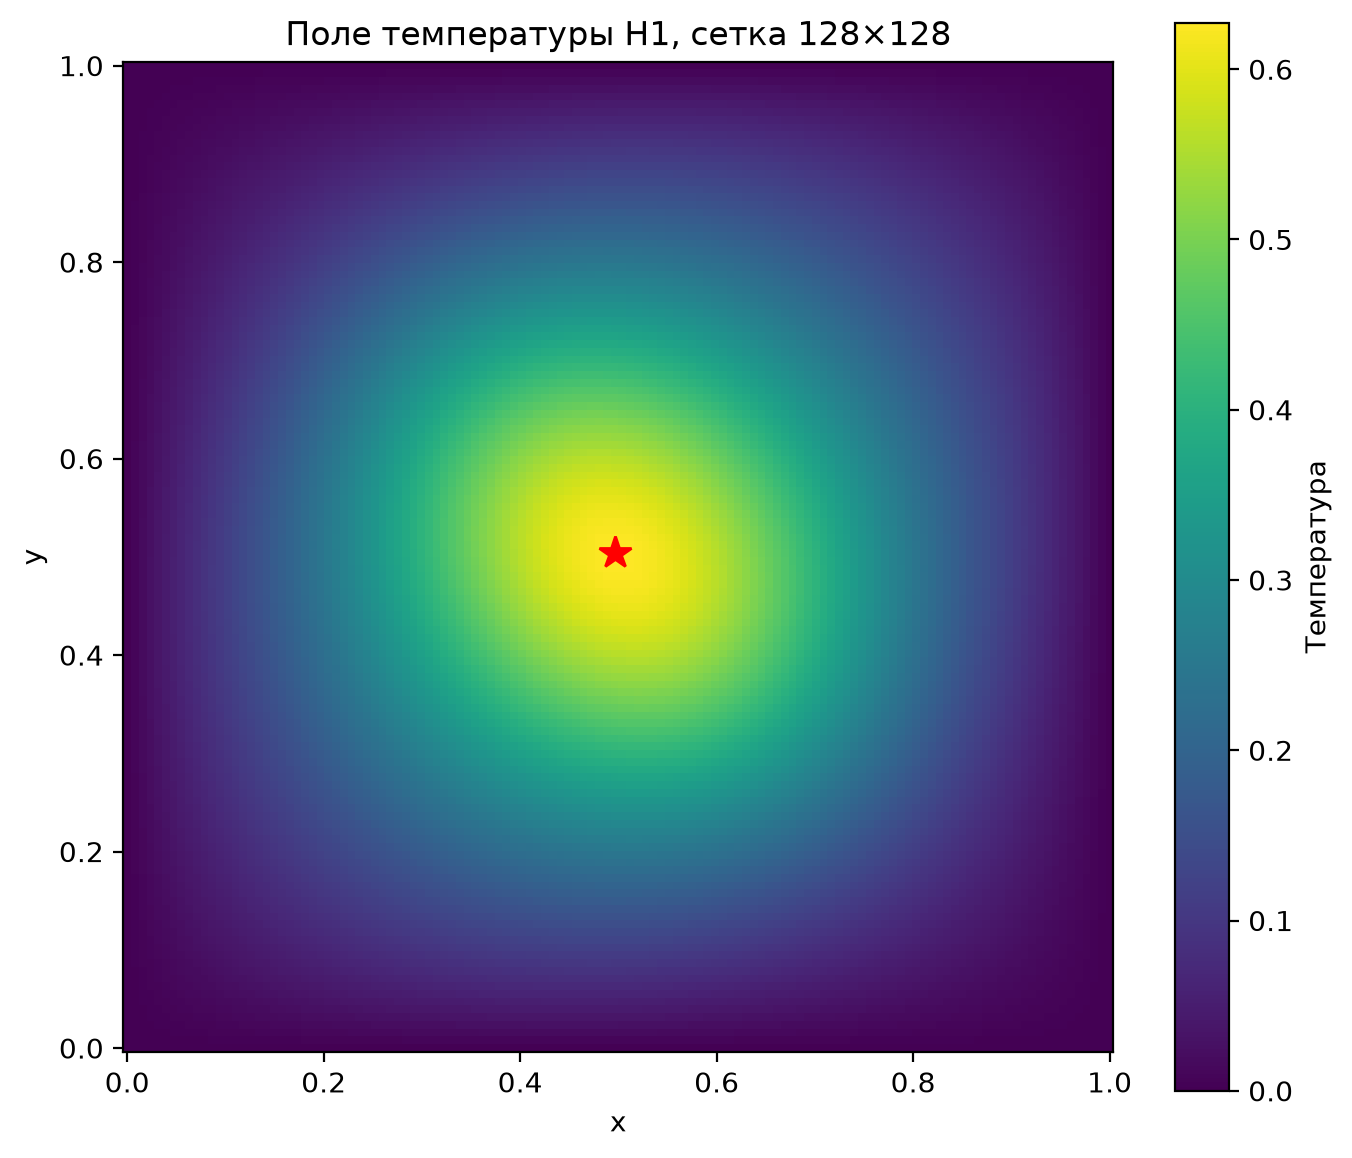
\includegraphics[width=\linewidth]{figures/temperature_field.png}
        \caption{Поле температуры на сетке $N=128$.}
    \end{subfigure}
\end{figure}

На сетке $N=128$ найден максимум температуры
$u_{\max}=\mathbf{0.62722526}$ в узле с координатами примерно $(0.4961,\,0.5039)$.

\section{Выводы}
С увеличением $N$ размер СЛАУ и число обусловленности растут, поэтому стационарные методы требуют существенно больше итераций. SSOR-PCG при отдельно подобранном $\omega=1.7067$ уменьшает их число до 51 при $N=128$ против 311 у CG, но два треугольных решения на шаг делают его медленнее: 98.0 мс против 34.1 мс. Наиболее быстрым в данных замерах оказался диагональный PCG (31.5 мс). Все запуски достигли порога, стагнации не наблюдалось.

\end{document}